%%% jetImp.tex
\documentclass[tikz]{standalone}
\usepackage{mdsTikz}
% Camera angles
\newcommand{\polarAngle}{60}
\newcommand{\aziAngle}{30}
%
\newcommand{\jetRad}{1.0}
\newcommand{\overJetRad}{1.0}
\newcommand{\maxRad}{4.5}
\newcommand{\jetHeight}{6.0}
\begin{document}
  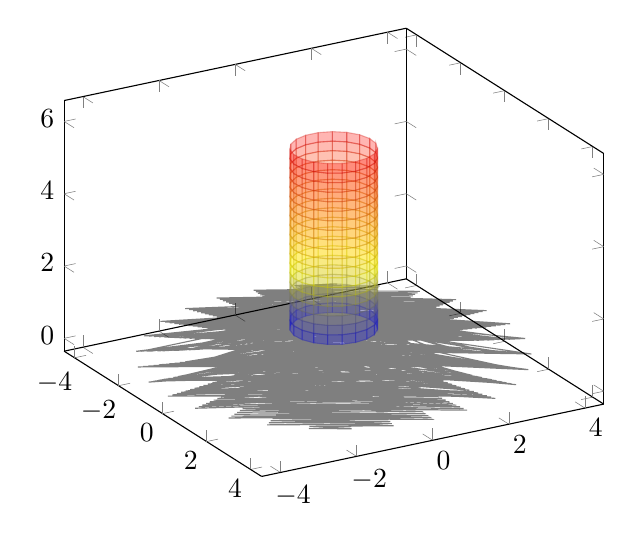
\begin{tikzpicture}
    \begin{axis}[view={\polarAngle}{\aziAngle}]
      \addplot3[
        opacity = 0.5,
        samples=30,
        domain=\jetRad:\maxRad,y domain=0:2*pi,
        z buffer=sort,
        axis x line*=none,
        axis y line*=none,
        axis z line*=none,
        xtick=\empty, ytick=\empty
        ]
        ({x*cos(deg(y))}, {x*sin(deg(y))}, {1/x});
      \addplot3[opacity=0.3,
                surf,
                no markers,
                clip=false,
                samples=20,
                domain=\overJetRad:\jetHeight,y domain=0:2*pi,
                z buffer=sort,
               ]
        ({\jetRad*cos(deg(y))}, {\jetRad*sin(deg(y))}, {x});
    \end{axis}
  \end{tikzpicture}
\end{document}

